\documentclass[11pt,a4paper]{report}
\usepackage[utf8]{inputenc}
\usepackage{amsmath}
\usepackage{amsfonts}
\usepackage{amssymb}
\usepackage[utf8]{inputenc}
\usepackage[T1]{fontenc}
\usepackage{textcomp}
\usepackage{gensymb}
\usepackage{graphicx}
\begin{document}

\subsection{Light direction independent scattering distribution}

In order to do importance sampling, we need to know the characteristics of the scattering distribution. More specifically, we need to know the amount of light from any incident direction $\omega_i$ that scatters to the viewer in direction $\omega_r$. If we know what incident light directions are important, we can find a sampling function that fits the shape of the scattering distribution. In figure~\ref{numstrands0} and figure~\ref{numstrands2} the scattering distribution is shown for different settings of $\omega_r$ and a constant number of hair strands $n_h$. These graphs show the difference between shading points that are directly illuminated and shading points that are indirectly illuminated.

\begin{figure}[h]
\begin{center}
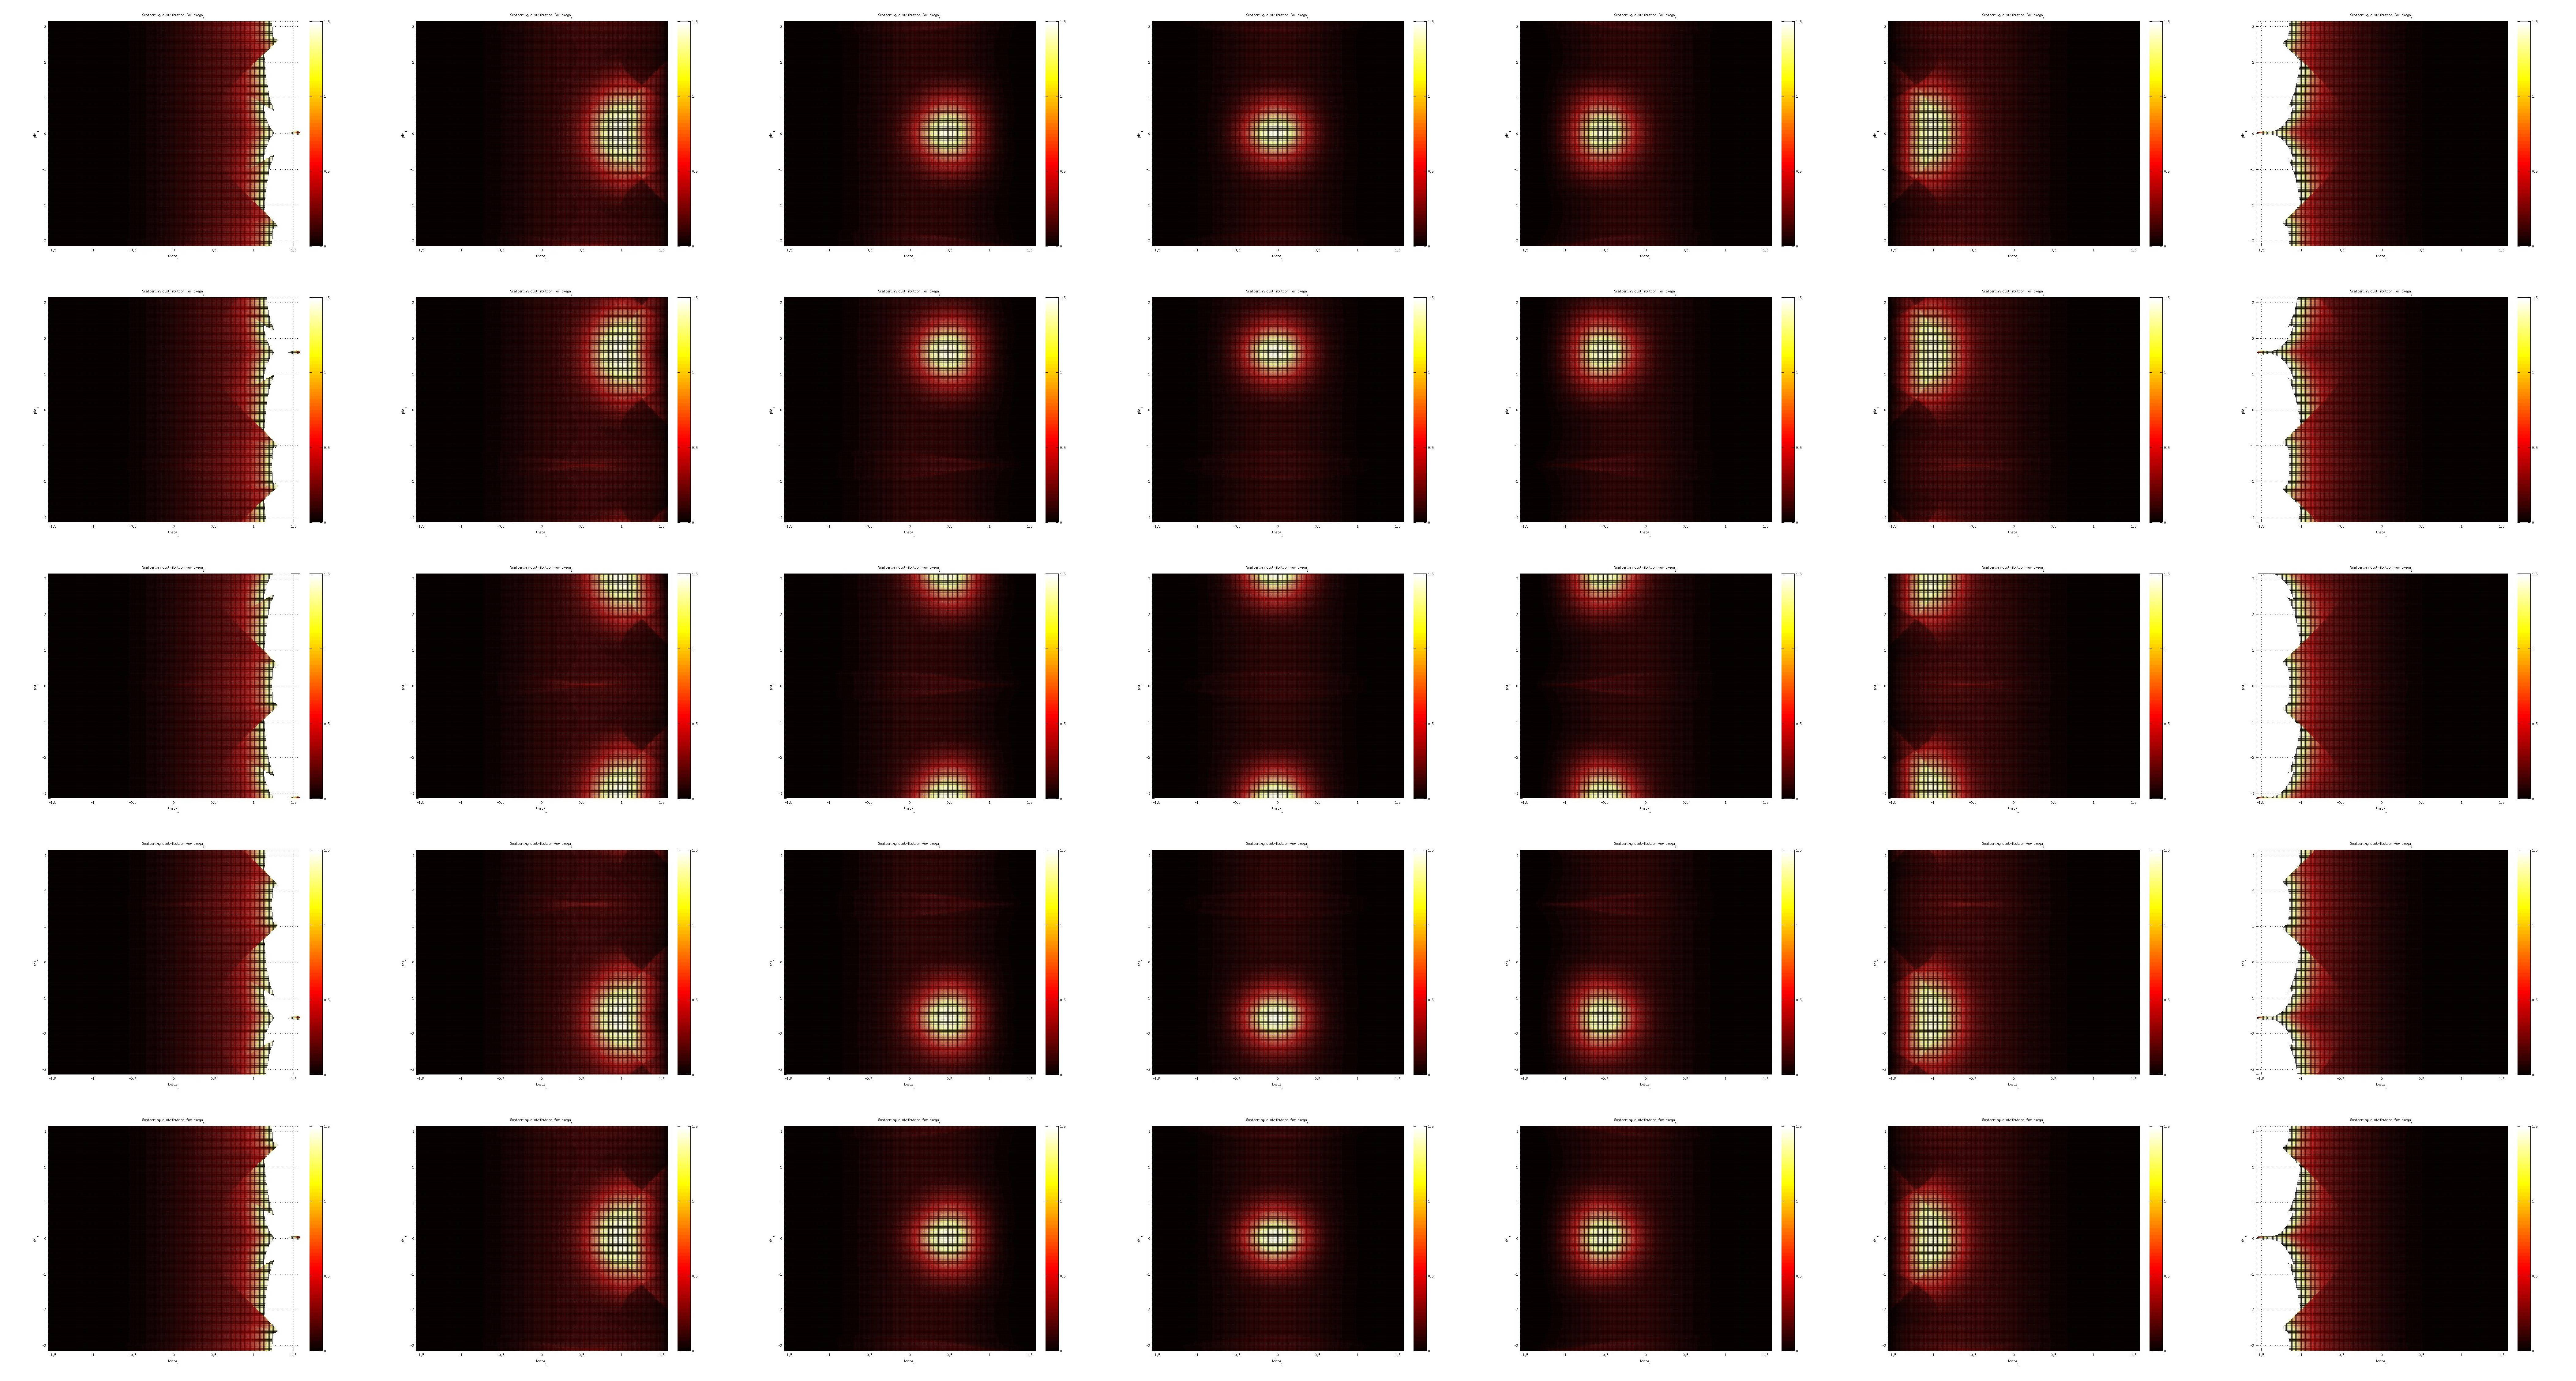
\includegraphics[scale=0.04]{images/scatteringdistribution/numstrands0.jpg}
\caption{The scattering distribution when no hair strands are between the viewer and the shading point (direct scattering). Each graph represent a different setting for $\omega_r = (\theta_r, \phi_r)$. Going from left to right (7 graphs), the value of $\theta_r$ is -90, -60, -30, 0, 30, 60 and 90 degrees. Going from top to bottom (5 graphs), the value of $\phi_r$ is 180, 90, 0, -90 and -180 degrees. Each of the smaller graphs represent variations in $\omega_i = (\theta_i, \phi_i)$. In this way, the collection of graphs show what incident light directions have a strong contribution for different directions of the viewer $\omega_r$.}
\label{numstrands0}

\end{center}
\end{figure}

\begin{figure}[h]
\begin{center}
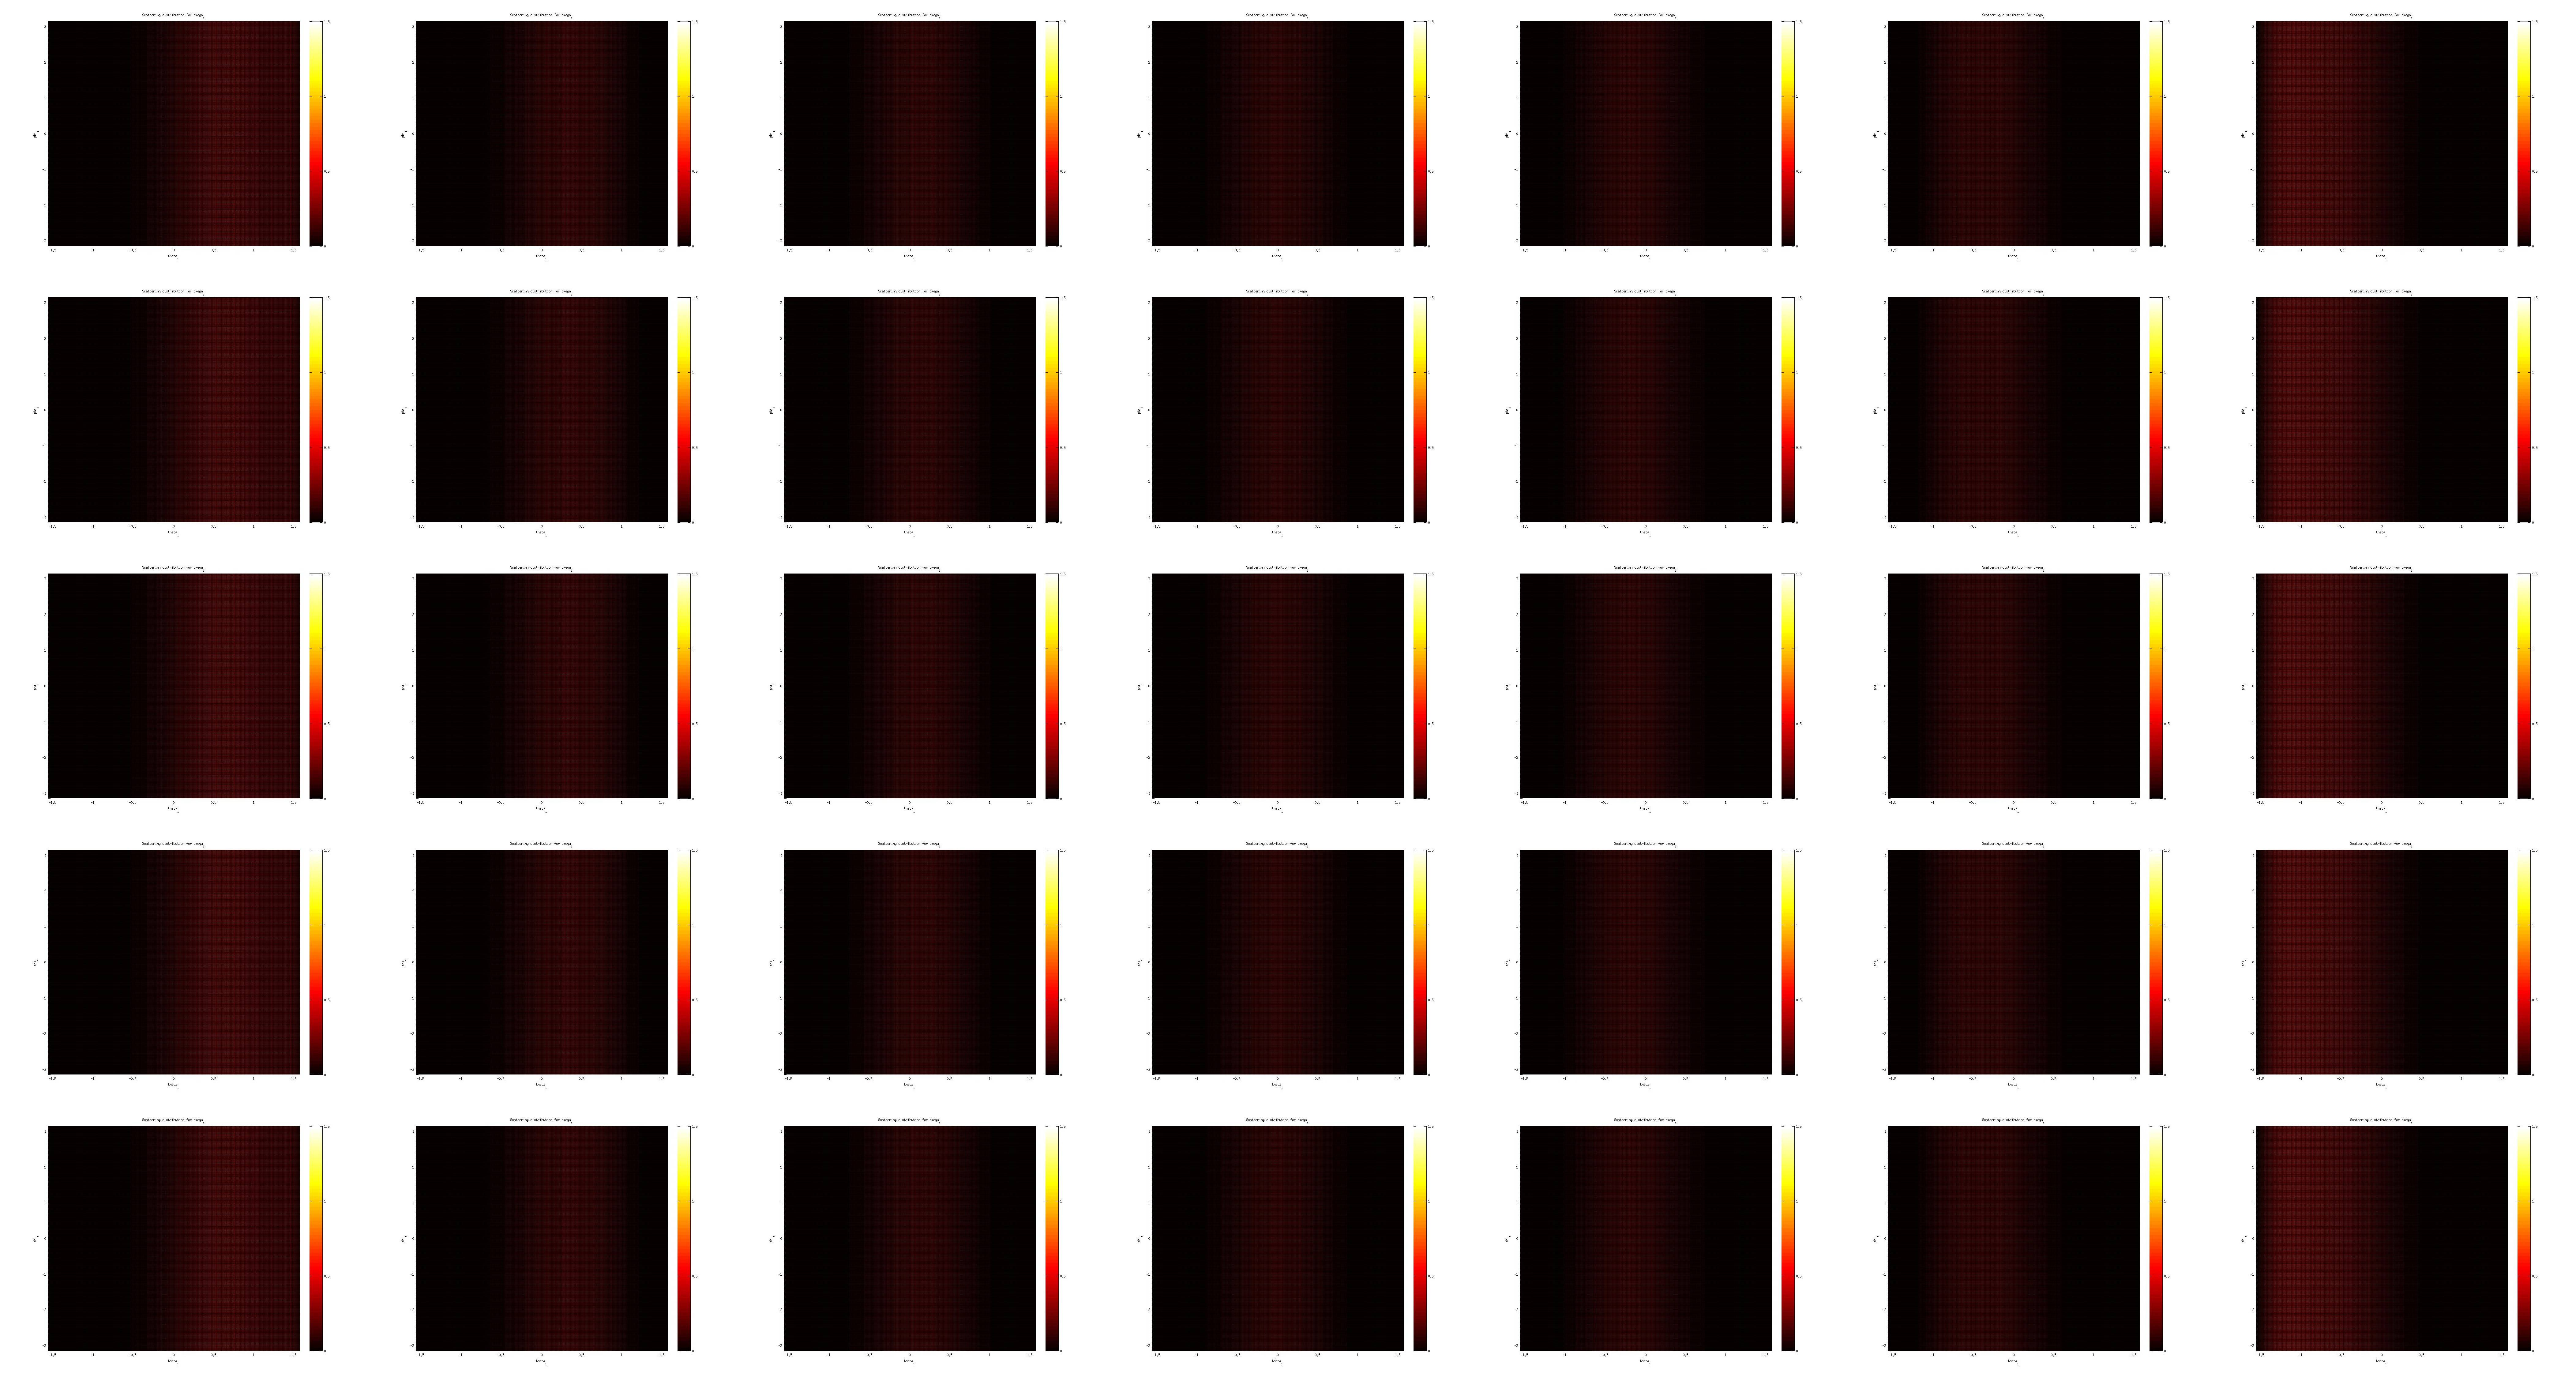
\includegraphics[scale=0.04]{images/scatteringdistribution/numstrands2.jpg}
\caption{Similarly to figure~\ref{numstrands0}, this graph depicts the same information but now for two hair strands (indirect scattering).}
\label{numstrands2}

\end{center}
\end{figure}


\subsubsection*{Conclusions from the graphs}

There are three observations to be made by looking at the graphs:

\begin{itemize}
\item Whenever the angle between the viewer and the hair fiber is almost parallel ($\theta_r \approx \pm 90$) degrees and the incident light direction $\theta_i$ is also close to $\pm 90$ degrees, but opposite to the viewer direction ($\theta_i \approx -\theta_r$), then the response is huge. Direct scattering resembles the Marschner model and this model has a strong reflection component, slightly tilted by a few degrees from the normal plane of the hair fiber. So this phenomenon is explainable. The value inside the data file shows that it goes up to 100. This is possible as long as the integration sums up to at most 1. The Marschner model is never claimed to be energy conserving, so it probably wouldn't obey this rule.

\item The second observation is the strong transmission component visible in the direct scattering distribution. From Marschner et al.~\ref{marschner} we know that the TT component is the most dominant component. The transmission component represents itself as a lobe, visible as an elliptical shape. This transmission lobe rotates around the hair fiber, directly opposite to $\phi_r$. So if $\phi_r = 0$ degrees, then the highlight is at $\phi_i = 180$ degrees. 

\item The third observation is the presence of a wide band of important directions spread over a range of $\theta_i$ angles. It is visible for the indirect scattering distribution, but also in the direct scattering distribution if you look behind the dominant lobe. The azimuthal direction does not play a role in this case, because the azimuthal distribution seems to be isotropic. As light propagates through more hair fibers, then eventually the longitudinal distribution should become isotropic as well. In that case, sampling is best done using uniform sampling.
\end{itemize}

The direct scattering graph shows artefacts inside the graph. This comes from the $N_R$, $N_{TT}$ and $N_{TRT}$ component. Why this is, is not clear yet.
[TO DO]: Fix this and remove text\\
 
The scattering distributions inside figure~\ref{numstrands0} and figure~\ref{numstrands2} essentially display the probability density function (PDF) for a range of viewing directions $\omega_r$. It shows which incident light directions contribute in what amount to the rendering result. To be able to do importance sampling, we need a way to sample incident light directions proportional to their importance. The important samples are the incident directions $\omega_i$ that are brightly colored inside the graph.

To do this, the PDF should be integrated to a normalized CDF. This graph, for example, has the $\theta_i$ on the $X$-axis. The vertical $Y$-axis starts at $Y=0$, and eventually integrates to $Y=1$ when all samples have been incorporated in the graph. If we invert the CDF, then the $\theta_i$ is on the $Y$-axis and the values 0 to 1 on the horizontal $X$-axis. Now we can just sample a random number between 0 and 1, and lookup the $\theta_i$ that belongs to it. In this way, the lobe represents a bigger part of the domain and is thus, more likely to be sampled.\\

Before we can integrate a PDF, we should first find a PDF. Finding a good PDF is the most important step in efficient importance sampling.

\subsubsection{Finding a probability density function (PDF)}

The observations that are made for the scattering distribution graphs boil down to two specific phenomena. The first one is the elliptical shape, or lobe, that is visible in the graphs for the direct scattering scenario. The other phenomena is primarily visible in the multiple scattering scenario, but also apparent in the direct scattering case, and is the wide band of directions that are uniform for the azimuthal angles and slightly dependent on the longitudinal angles.

These two phenomena can each be described using it's own probability density function (PDF). The PDF $f(\omega_i, \omega_r)$ returns the probability that incident light direction $\omega_i$ is sampled, given the direction to the viewer $\omega_r$. Since it is hard to find a single function that combines both the direct and indirect scattering scenarios, it is better to split up the PDF $f(\omega_i, \omega_r)$ into two separate functions. One for the direct scattering case $f_{ds}$ and one for the multiple scattering case $f_{ms}$. When doing importance sampling we can divide the number of samples between both PDF. The idea is that by using separate PDFs we still obtain faster rendering times, compared to uniform sampling.

\subsubsection{The direct scattering PDF}

The direct scattering probability density function (PDF) $f_{ds}(\omega_r, \omega_i)$ can be described by a combination of two Gaussian functions. Each of these functions describes the shift of the lobe along the horizontal and the vertical axes. The PDF for the direct scattering function will be as follows:

\begin{equation}
f_{ds}(\omega_i, \omega_r) = f_{ds}^L(\omega_i, \omega_r) \cdot f_{ds}^A(\omega_i, \omega_r)
\end{equation}

\begin{itemize}
\item A function $f_{ds}^L(\omega_i, \omega_r)$ explaining the shift of the lobe along the horizontal axis (longitudinal angle).

\item Another function $f_{ds}^A(\omega_i, \omega_r)$ describes the shift along the vertical axis (azimuthal angle).
\end{itemize}

A different value for $\theta_r$ causes the lobe to be shifted sideways. It turns out as $\theta_r$ increases in value, then the lobe is shifted in the other direction by the same amount of degrees for $\theta_i$. More concrete, this means that the lobe is positioned at the location where $\theta_i = -\theta_r$, or also described as $\theta_i + \theta_r = 0$. \\

With this knowledge we can find the longitudinal part of the direct scattering PDF. A Gaussian function has the following general form:

\begin{equation}
a \cdot \exp \Big ( -\frac{(x - b)^2}{2c^2} \Big ) + d 
\end{equation}

A normalized Gaussian function $g(\mu, \sigma)$ with mean $\mu$ and standard deviation $\sigma$ fills in these values as follows:

\begin{align}
a &= \frac{1}{\sigma \cdot \sqrt{2 \pi}} \\
b &= \mu \\
c &= \sigma \\
d &= 0 \\
\end{align}

The center of the lobe is positioned at $\mu = 0$, meaning that $b = 0$. The standard deviation $\sigma$ describes how wide the lobe is. Smaller standard deviations lead to narrow lobes and larger peaks. Likewise, larger standard deviations lead to wider lobes and smaller peaks. By trying to match the width of the normalized Gaussian function to the width of the lobe in the scattering distribution graph, it turns out that $\sigma = 0.22$ works well. Now we can describe the longitudinal part of the direct scattering PDF $f_{ds}^L$:


\begin{align*}
\sigma &= 0.44 \\
 f_{ds}^L(\theta_r, \theta_i) &= \frac{1}{\sigma \cdot \sqrt{2 \pi}} \cdot \exp \Big ( -\frac{(\theta_i + \theta_r)^2}{2 \sigma^2} \Big ) \\
\end{align*}


The azimuthal component of the direct scattering PDF $f_{ds}^A$ is found in a similar fashion as the longitudinal variant. The lobe is now centered at the opposite end of the fiber, because of the nature of the transmission component. That means that the lobe is centered at $\phi_i + \phi_r = \pm 2\pi$ (or $\pm$ 180 degrees). 

Since the lobe seems to stretch in the vertical direction as $\theta_r$ becomes larger, with its maximum stretch at $\theta_r = \pm \frac{1}{2} \pi$, this stretch should be incorporated in the PDF. The standard deviation $\sigma$ is used to control the width of the lobe, so by attaching a parabolic function $r(\theta_r)$ to $\sigma$ based on $\theta_r$, we can have a stretching lobe as $\theta_r$ comes closer to $\pm$ 90 degrees. By matching the shape of the stretch with the scattering distribution graphs, we obtain the following azimuthal component of the direct scattering PDF: 

\begin{align*}
r(\theta_r) &= \frac{\theta_r}{\pi} \\
\sigma &= 0.52 + r^2 \\
 f_{ds}^A(\phi_r, \theta_r, \phi_i) &= \frac{1}{\sigma \cdot \sqrt{2 \pi}} \cdot \exp \Big ( -\frac{(\phi_i + \phi_r \pm 2\pi)^2}{2 \sigma^2} \Big ) \\
\end{align*}

If we write out the equations for both the longitudinal and the azimuthal scattering equation we obtain the following PDF for the direct scattering component:

\begin{equation}
f_{ds} = f_{ds}^L \cdot f_{ds}^A
\end{equation}



\subsubsection{Multiple scattering sampling function}

The multiple scattering scenario requires us to find a PDF for different number of hair strands $n_h$. A consideration to be made is whether it is important to make a distinction based on the number of hair strands between the shading point and the light source. Ideally we should take it into consideration, but if after only a few scattering events the distribution is already isotropic, then we might just as well use uniform sampling and not care about the small fraction of samples that might be devoted to situations with only one, two or three scattering events.

As long as the distribution is not isotropic, we can approximate the scattering distribution graph with a Gaussian function, in the same way as we did for the direct scattering scenario. Multiple scattering is only dependent on the longitudinal angles $\theta_i$ and $\theta_r$, because it is isotropic for azimuthal angles. This makes the PDF much simpler compared to the direct scattering variant.


\begin{figure}[h]
\begin{center}

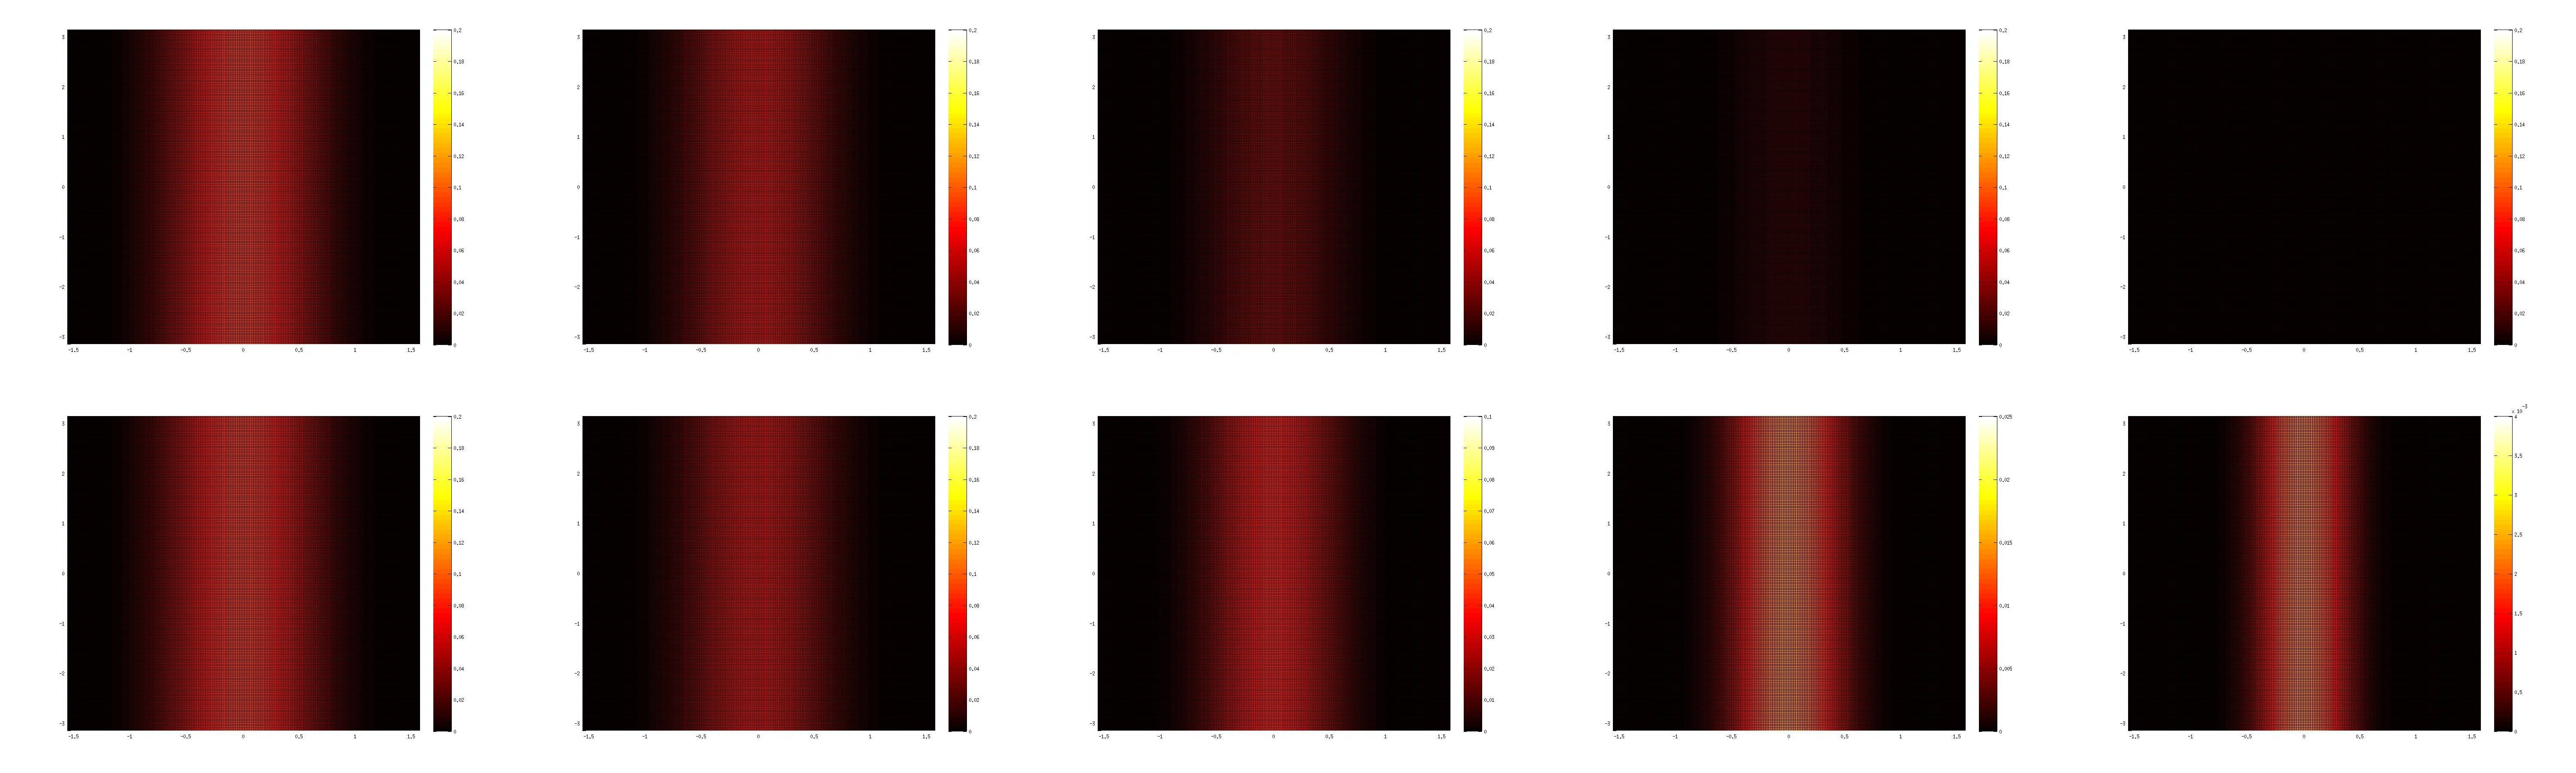
\includegraphics[scale=0.06]{images/scatteringdistribution/multiplescattering_bandwidth_lowres.jpg}

\caption{A series of images for $\theta_r = 0$ that show the width of the band  and with different number of hair strands. Here you can see how the width of the band varies as the number of hair strands increase. The top row keeps the color scale between 0 and 0.2, with 0.2 being white, and 0 being black. The bottom row shows the same image sequence but with a varying color scale. In this way the shape of the bands is clearly visible. It is clear to see that the amount of scattering decreases as the number of hair strands increase. From left to right, the number of hair strands are: 1, 2, 4, 8, 16.}
\label{bandwidth}
\end{center}
\end{figure}

Figure~\ref{bandwidth} shows an image sequence for the multiple scattering situation for different number of hair strands. As the number of hair strands increase, more and more light will be absorbed leading to a darker rendering result. Also, as the number of strands increase, the width of the band decreases. In table~\ref{stddev_settings_for_number_of_hairstrands} the standard deviations are shown for different number of hair strands. These values are found by experimentation and try to make the Gaussian function as wide as the width of the bands visible in figure~\ref{bandwidth}.\\

\begin{table}[h]
\begin{center}
\begin{tabular}{l|c|c|c|c|c}
Number of hair strands $n_h$ & 1 & 2 & 4 & 8 & 16 \\
\hline
Standard deviation $\sigma$ & 0.44 & 0.41 & 0.37 & 0.34 & 0.29 \\
\end{tabular}
\caption{A Gaussian function is used to describe the bands in the scattering distribution. The width of the Gaussian function is controlled by the standard deviation $\sigma$. As the number of hair strands $n_h$ increases through which light scatters, then the width of the band increases and requires larger standard deviations so that the Gaussian function mimics the band. Eventually the distribution will be pretty much isotropic. This graph shows suitable standard deviation settings for different number of hair strands.}
\label{stddev_settings_for_number_of_hairstrands}
\end{center}
\end{table}

As $\theta_r$ increases, the band is shifting in the other direction by the same amount in the $\theta_i$ direction. This means that the peak of the Gaussian is exactly at the position where $\theta_i + \theta_r = 0$. The width of the lobe is not only dependent on the number of hair strands, but also on $\theta_r$. As $\theta_r$ increases, the lobe becomes wider and thus the standard deviation should increase as well. The amount that the standard deviation should change depends on $\theta_r$ and so the adjustment can be captured in a function $r(\theta_r)$. If we compute the adjustment as a ratio between between $[-\pi/2 ; \pi/2]$ and then divide by 2, we can describe the multiple scattering PDF as follows:

\begin{align}
r(\theta_r) &= \frac{1}{2} \cdot \frac{2 \cdot \theta_r}{\pi} = \frac{\theta_r}{\pi}\\
\sigma' &= r(\theta_r) + \sigma \\
f_{ms}(\theta_i, \theta_r) &= \frac{1}{\sigma' \cdot \sqrt{2 \pi}} \cdot \exp \Big ( -\frac{(\theta_i + \theta_r)^2}{2 \sigma'^2} \Big )
\end{align}

\subsection{Fitting the Gaussian functions}

The scattering distribution shows which incident light directions $\omega_i$ are preferred to be sampled for a given viewer direction $\omega_r$. To be able to sample a direction, three steps should be performed. 

\begin{enumerate}
\item A probability density function (PDF) should be created that accurately matches the scattering distribution.
\item The PDF needs to be integrated to a normalized cumulative distribution function (CDF).
\item The CDF needs to be inverted to an inverted CDF.
\end{enumerate}

In this section, the creation of the PDF is explained. The PDF should  accurately match the scattering distribution. The more accurate it matches the distribution, the better the sampling will become. Since the scattering distribution differs between directly illuminated strands, versus indirectly illuminated strands, a choice is made to create two different probability density functions that are combined together. These are the direct scattering PDF and the multiple scattering PDF.



 The direct scattering is more complex to be matched. 

\subsubsection{Fitting the direct scattering distribution}

\subsubsection{Fitting the multiple scattering distribution}


For the multiple scattering scenario, the likelihood of a direction $\omega_i$ to be sampled is only dependent on the longitudinal directions $\theta_r$ and $\theta_i$. The shape looks a lot like a Gaussian function and therefore the distribution is matched by using a single normalized Gaussian function.

In order to fit the Gaussian functions to the scattering distribution, we will need to adjust the mean and the standard deviation to find an accurate match. Table~\ref{optimal_values} shows optimal values for different orientations of the viewer $\theta_r$. As light scatters through multiple fibers, light is absorbed leading to a smaller response. For this reason, a scale factor is introduced so that the normalized Gaussian function can be scaled up or down to match the scattering distribution. Eventually the scale factor is ignored in the PDF, because for the sampling process, the scale factor is not relevant. Since we need a normalized PDF, we can ignore the scale factor and still have a PDF that matches the shape of the scattering distribution.

\begin{table}[h]
\begin{center}
\begin{tabular}{|cc|c|c|c||cc|c|c|c|}
\hline
\# strands & $\theta_r$ & $s$ & $\sigma$ & $\mu$-shift  & \# strands & $\theta_r$ & $s$ & $\sigma$ & $\mu$-shift\\ \hline \hline
1 & -90 & $1$ & $0.75$ & $0 \degree$					& 2 & -90 & $\frac{4}{10}$ & $0.90$ & $0\degree$ \\
  & -60 & $\frac{10}{67}$ & $0.55$ & $-34.5 \degree$ 	&  & -60 & $\frac{100}{965}$ & $0.55$ & $-38\degree$ \\
  & -30 & $\frac{1}{9}$ & $0.49$ & $-20 \degree$ 		&  & -30 & $\frac{1}{12}$ & $0.49$ & $-20\degree$ \\
 & 0 & $\frac{2}{19}$ & $0.49$ & $-1.2\degree$ 			&  & 0 & $\frac{10}{125}$ & $0.49$ & $-1.2\degree$ \\
 & 30 & $\frac{1}{9}$ & $0.49$ & $17.5 \degree$ 			&  & 30 & $\frac{1}{12}$ & $0.49$ & $17.5\degree$ \\

   & 60 & $\frac{10}{67}$ & $0.55$ & $29 \degree$ 		&  & 60 & $\frac{100}{965}$ & $0.55$ & $34\degree$ \\

  & 90 & $2$ & $0.65$ & $0 \degree$ 					&  & 90 & $\frac{4}{10}$ & $0.90$ & $0\degree$ \\ \hline
4  & -90 & $\frac{1}{15}$ & $0.51$ & $-61 \degree$					& 8 & -90 & $\frac{1}{60}$ & $0.41$ & $-70\degree$ \\
  & -60 & $\frac{10}{205}$ & $0.47$ & $-43 \degree$ 	&  & -60 & $\frac{1}{70}$ & $0.38$ & $-49\degree$ \\
  & -30 & $\frac{1}{25}$ & $0.41$ & $-22 \degree$ 		&  & -30 & $\frac{1}{73}$ & $0.38$ & $-25\degree$ \\
 & 0 & $\frac{10}{255}$ & $0.41$ & $-1.2\degree$ 			& & 0 & $\frac{1}{78}$ & $0.36$ & $-1.2\degree$ \\
 & 30 & $\frac{1}{25}$ & $0.41$ & $20 \degree$ 			&  & 30 & $\frac{1}{75}$ & $0.38$ & $23\degree$ \\
 & 60 & $\frac{10}{205}$ & $0.47$ & $40 \degree$ 		&  & 60 & $\frac{1}{73}$ & $0.38$ & $46\degree$ \\
 & 90 & $\frac{1}{14}$ & $0.52$ & $54 \degree$ 					&  & 90 & $\frac{1}{63}$ & $0.41$ & $68\degree$ \\ \hline
\end{tabular}
\caption{For every longitudinal angle $\theta_r$ and number of hair strands, the optimal standard deviation $\sigma$, shifted mean ($\mu$) and scale factor is displayed so that the normalized Gaussian function matches the scattering distribution. The scale factor is eventually ignored, because it is not important for the PDF.}
\label{optimal_values}
\end{center}
\end{table}

Figure~\ref{fitting} shows the fitting of the Gaussian functions for multiple scattering through 1, 2, 4 and 8 fibers. As can be seen is that the Gaussian functions match pretty well. As $\theta_r$ increases, the distribution becomes narrower on one of the sides. The Gaussian function does not take this into account. Choosing a PDF is a compromis between a function that matches the underlying PDF pretty well, and should be easy to integrate and evaluate. If the function becomes too expensive to evaluate, then uniform sampling might be more efficient after all.


\begin{figure}[h]
\begin{center}
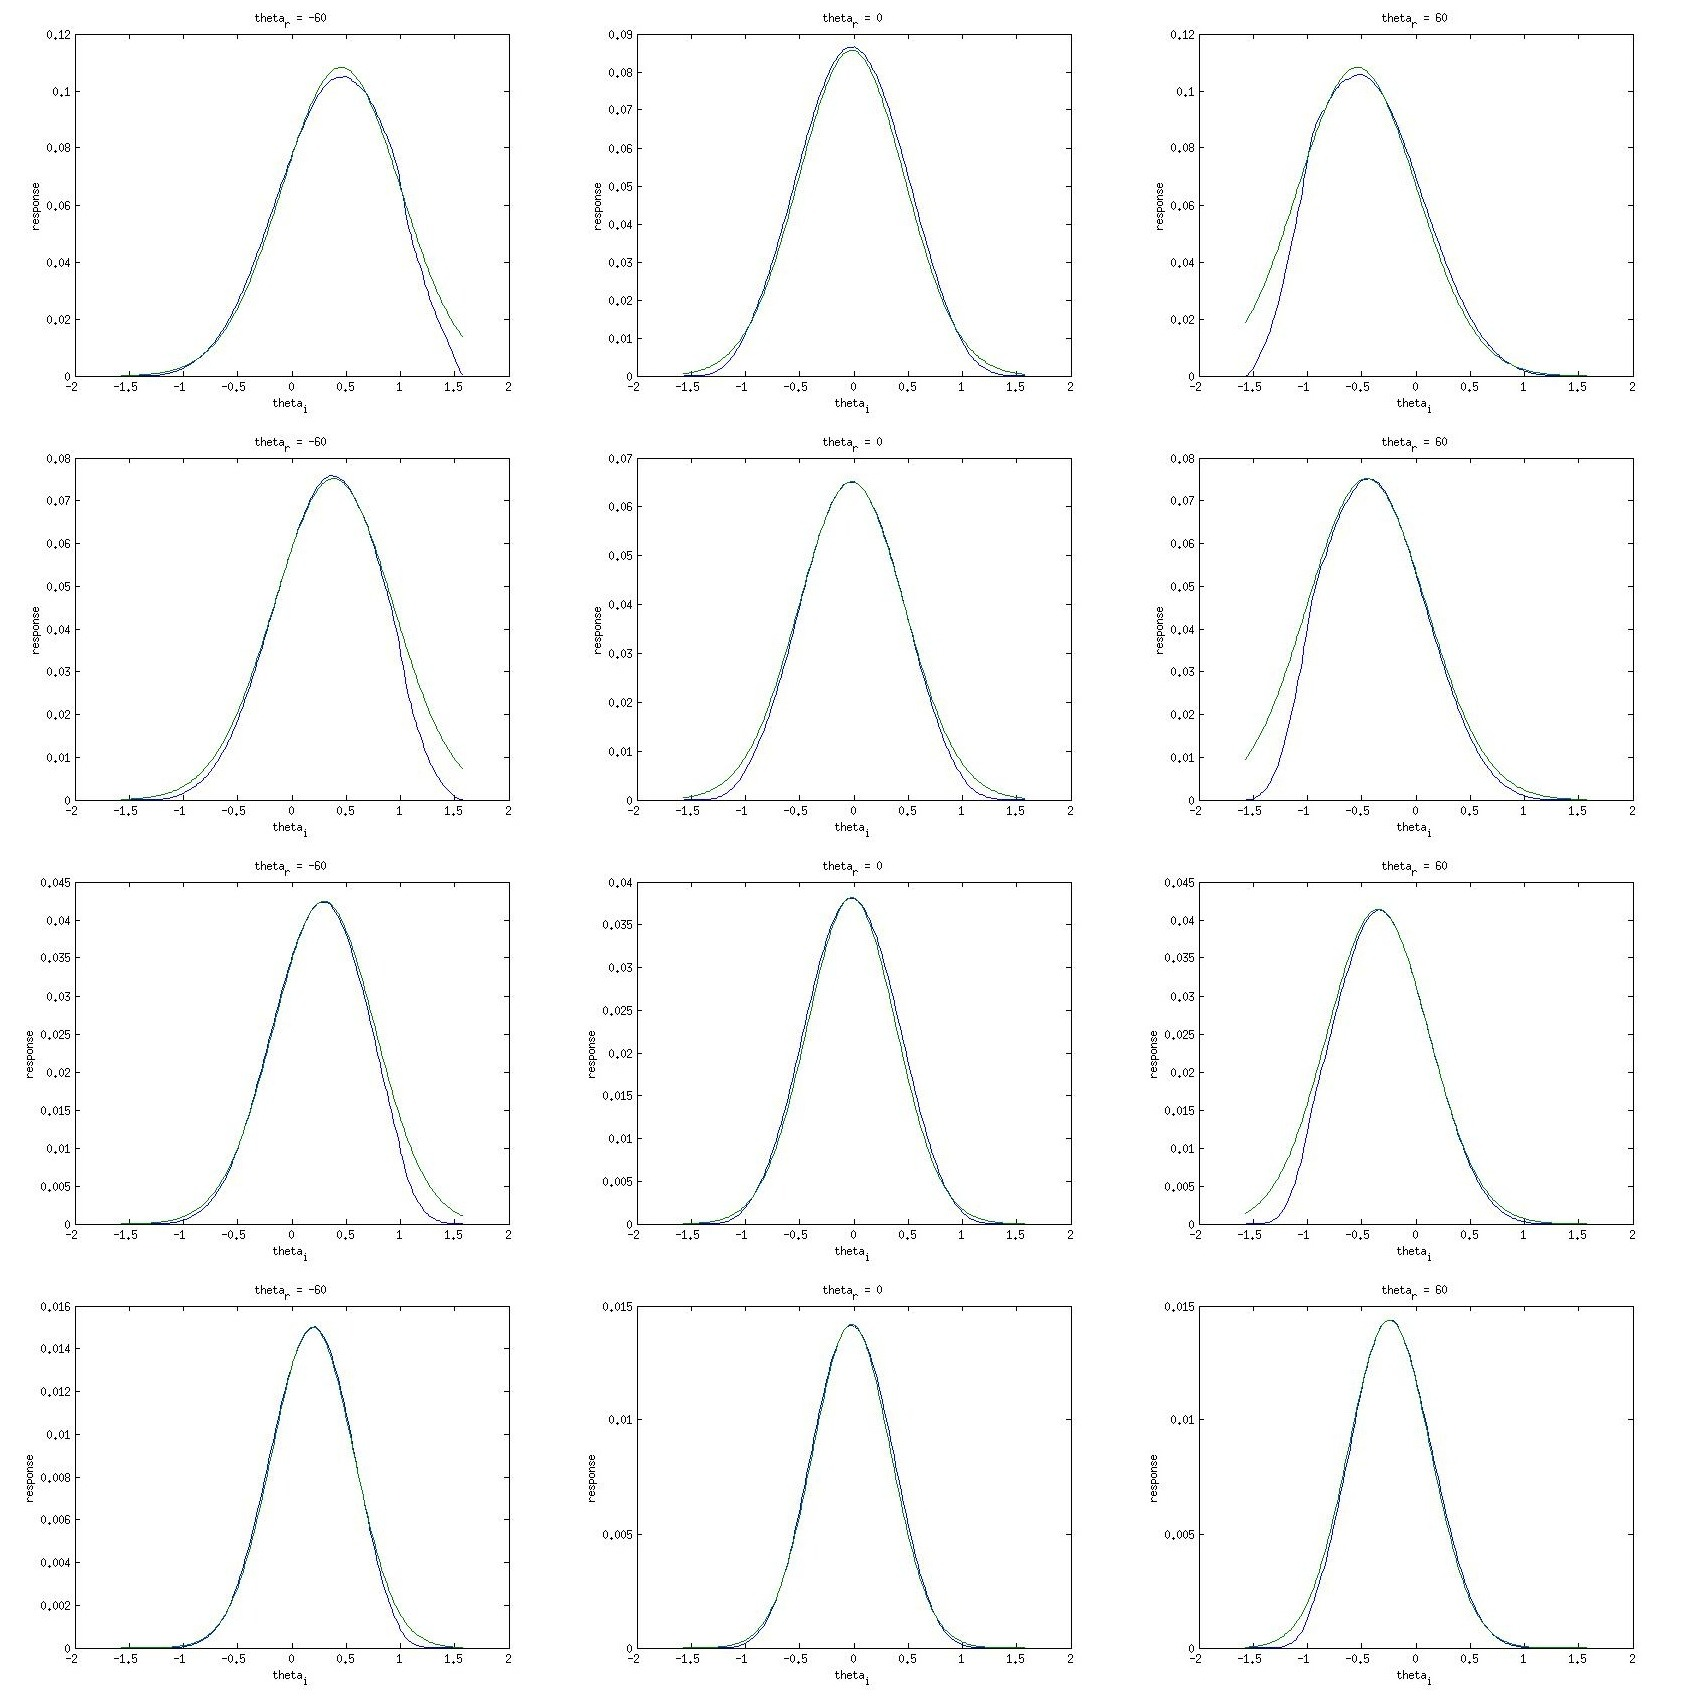
\includegraphics[scale=0.20]{images/graphfitting/fitting_combined.jpg}
\caption{A 2D slice of the scattering distribution for different number of hair strands that the light scatters through versus different $\theta_r$ (-60, 0 and 60 degrees). The top row corresponds to 1, the second to 2, the third to 4 and the last row to 8 number of hair strands. The scattering distribution is shown in blue and the created Gaussian function is green.}
\label{fitting}

\end{center}
\end{figure}





\subsection{Comparing the scattering distribution with the generated distribution}



\end{document}